\documentclass[12pt]{article}
\usepackage{fullpage,amsfonts,amssymb,epsfig,amsmath,hyperref,mdframed, graphicx}
\usepackage{caption, parskip, array, listings}
\newenvironment{gamequote}
               {\list{}{\rightmargin0pt\relax}\item\relax}%
               {\endlist}

\newcommand{\half}{{1 \over 2}}
\newcommand{\xor}{{\oplus}}
\newcommand{\owf}{f}
\newcommand{\Sign}{\mathsf{Sign}}
\newcommand{\Verify}{\mathsf{Verify}}
\newcommand{\KeyGen}{\mathsf{KeyGen}}
\newcommand{\pk}{\mathit{pk}}
\newcommand{\adv}{\mathcal{A}}
\newcommand{\bdv}{\mathcal{B}}
\newcommand{\deq}{\mathrel{:=}}
\newcommand{\rgets}{\mathrel{\mathpalette\rgetscmd\relax}}
\newcommand{\rgetscmd}{\ooalign{$\leftarrow$\cr
    \hidewidth\raisebox{1.2\height}{\scalebox{0.5}{\ \rm R}}\hidewidth\cr}}
\newcommand{\Z}{\mathbb{Z}}
\newcommand{\F}{\mathbb{F}}
\newcommand{\R}{\mathbb{R}}
\newcommand{\G}{\ensuremath{\mathbb{G}}}
\newcommand{\GG}{\ensuremath{\mathbb{G}}}
\newcommand{\Zq}{\ensuremath{{\Z_q}}}
\newcommand{\sk}{\textrm{sk}}
\newcommand{\vk}{\text{vk}}
\newcommand{\lcat}{\langle}
\newcommand{\rcat}{\rangle}
\newcommand{\tuple}[1]{\lcat #1 \rcat}
\newcommand{\KK}{\mathcal{K}}  % key space
\newcommand{\XX}{\mathcal{X}}  % key space
\newcommand{\YY}{\mathcal{Y}}  % key space
\newcommand{\CC}{\mathcal{C}}  % key space
\newcommand{\MM}{\mathcal{M}}  % key space

\newcommand{\FlowRight}[2][200pt]{%
  \xrightarrow{\text{\normalsize\hbox to #1{\hfill \(#2\) \hfill}}}
}
\newcommand{\FlowLeft}[2][200pt]{%
  \xleftarrow{\text{\normalsize\hbox to #1{\hfill \(#2\) \hfill}}}
}


%%%%%%%%
\usepackage{enumitem}

\newenvironment{problems}
{\begin{enumerate}[label=\bfseries Problem \arabic*.,align=left,leftmargin=1em,labelwidth=1.5em]}
{\end{enumerate}}

\newenvironment{subparts}
{\begin{enumerate}[label=\bfseries \alph*.,align=right,leftmargin=1.5em]}
{\end{enumerate}}
%%%%%%%%

\begin{document}

\newlength{\boxwidth}
\setlength{\boxwidth}{\textwidth}
\addtolength{\boxwidth}{-2cm}
\framebox[\textwidth]{
\begin{minipage}[t]{\boxwidth}
{\bf CS155: Computer and Network Security \hfill Spring 2023}  \\[-0.3cm]
\begin{center} {\huge Homework \#1} \end{center}
Due: Thursday, Mar. 27, 2023, by Gradescope.
\end{minipage}}

\vspace{0.7cm}
\begin{problems}

%%%%%%%%%%%%%%%%%%%%%%%%%%%%%%%%%%%%%%%%%%%%%%%%%%%%%%%%%%%%%%
\item \textbf{Jump Oriented Programming (JOP)}

Elizabeth is attacking a buggy application. She has found a vulnerability that allows her to control the values of the registers ecx, edx, and eip, and also allows her to control the contents of memory locations 0x9000 to 0x9014. She wants to use return-oriented programming, but discovers that the application was compiled without any ret instructions! Nonetheless, by analyzing the application, she learns that the application has the following code fragments (gadgets) in memory: \\
\begin{verbatim}
0x3000: add edx, 4      ; edx = edx + 4
        jmp [edx]       ; jump to *edx

0x4000: add edx, 4      ; edx = edx + 4
        mov eax, [edx]  ; eax = *edx
        jmp ecx         ; jump to ecx

0x5000: mov ebx, eax    ; ebx = eax
        jmp ecx         ; jump to ecx

0x6000: mov [eax], ebx  ; *eax = ebx
        ...             ; don't worry about what happens after this
\end{verbatim}

Show how Elizabeth can set the values of the registers and memory so that the vulnerable application writes the value 0x2222 to memory address 0x8888.

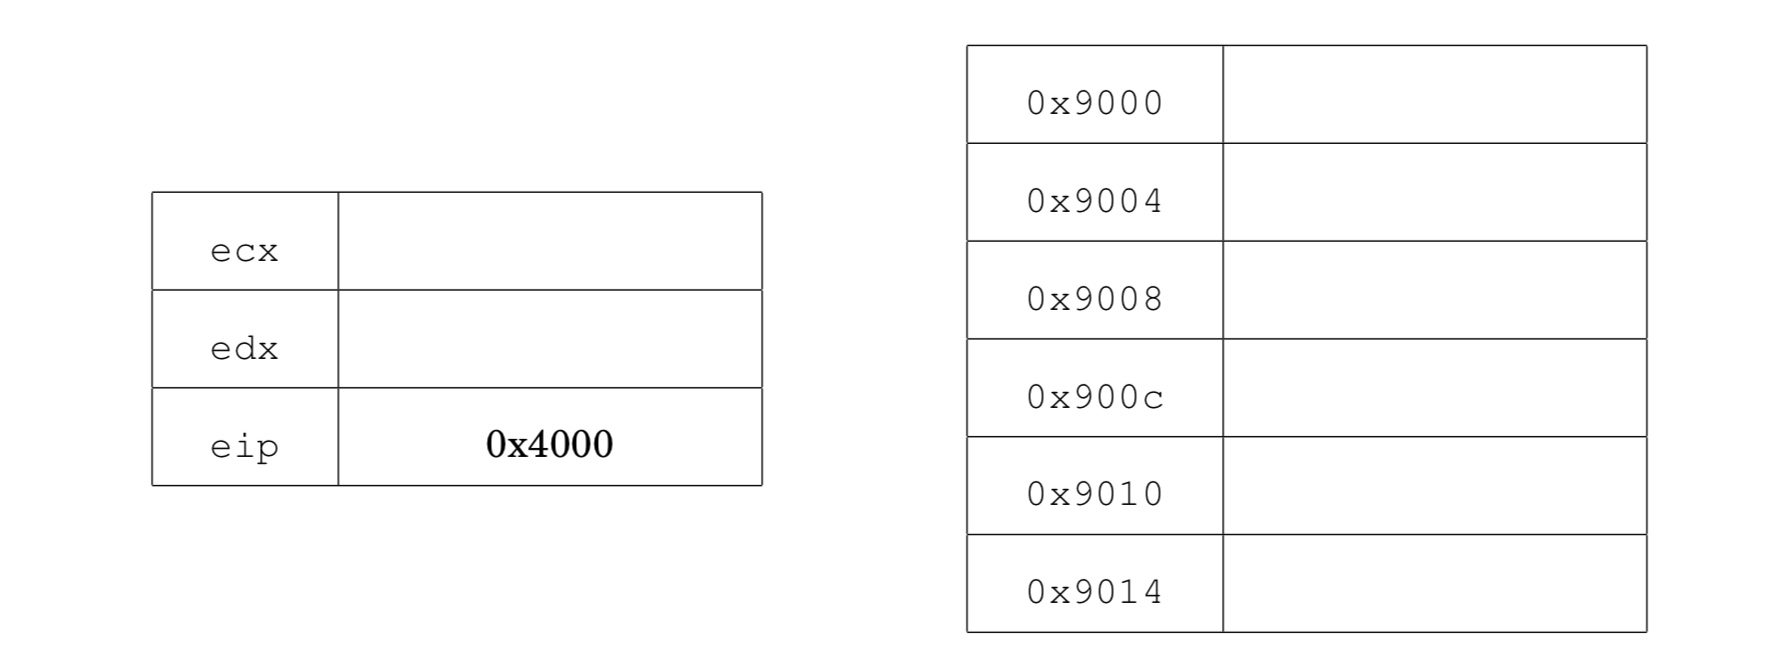
\includegraphics[scale=0.2]{jmp.jpg}

Recall that \texttt{eip} is the instruction pointer. It holds the address of the next instruction to execute. \texttt{ecx} and \texttt{edx} are general purpose registers.

\begin{mdframed}

    Idea: Want to set the registers and memory locations we have control over in such a way that we can execute \texttt{0x6000} with \texttt{eax = 0x8888} and \texttt{ebx = 0x222} respectively.
    To do this, we need to solve for how our "gadgets" can be daisy-chained together to get the desired result. 
    In particular, we line up our "gadgets" in the memory locations 0x9000-0x9014 and use \texttt{ecx = 0x3000} to iteratively jump from gadget to gadget.
    
    \begin{itemize}
        \item \textbf{Gadget 1}: We are given \texttt{eip = 0x4000} as the address of the first gadget. We need to set edx to determine which memory location is used to update the eax register. We know we want \texttt{ebx = 0x2222} by the time we call 0x6000, so let's pick \texttt{edx = 0x9000} and fill memory location \texttt{0x9004 = 0x2222}, which guarantees that \texttt{eax = *0x9004 = 0x2222} after this first gadget is executed (we will need to shift this value to ebx).
        \item \textbf{Gadget 2}: The last instruction of the first gadget is \texttt{jmp ecx}, and so our next gadget needs to be placed at the ecx register. Since we want to daisy-chain together our gadgets, we need to find a way to progressively iterate through memory locations. To do this, we set \texttt{ecx = 0x3000} which returns us to our memory stack, but four positions higher. Fill memory location \texttt{0x9004 = 0x5000} to ensure that \texttt{ebx = *edx = 0x2222} after this gadget is executed.
        \item \textbf{Gadget 3}: Again the last instruction from gadget 2 is \texttt{jmp ecx}, which increments edx by 4 and jumps back to *edx (memory location of our new gadget). We have set \texttt{0x900c = 0x4000}, which sets eax to be the value of edx + 4, which is the location of our next memory address! Let's set \texttt{0x90010 = 0x8888}, which updates \texttt{eax = 0x8888} as desired and jumps back to our iterator ecx.
        \item \textbf{Gadget 4}: Finally, we are ready to execute 0x6000 since both \texttt{eax = 0x8888} and \texttt{ebx = 0x2222} registers are prepared. We store 0x6000 at memory location 0x9014 and we are done.
    \end{itemize}

\end{mdframed}

\begin{table}[!htb]
    \begin{minipage}{.5\linewidth}
      \caption{registers}
      \centering
        \begin{tabular}{|l|l|}
            \hline
            ecx & 0x3000 \\ \hline
            edx & 0x9000 \\ \hline
            eip & 0x4000 \\ \hline
        \end{tabular}
    \end{minipage}%
    \begin{minipage}{.5\linewidth}
      \centering
        \caption{stack memory}
        \begin{tabular}{|l|l|}
            \hline
            0x9000 &        \\ \hline
            0x9004 & 0x2222 \\ \hline
            0x9008 & 0x5000 \\ \hline
            0x900c & 0x4000 \\ \hline
            0x9010 & 0x8888 \\ \hline
            0x9014 & 0x6000 \\ \hline
        \end{tabular}
    \end{minipage} 
\end{table}

%%%%%%%%%%%%%%%%%%%%%%%%%%%%%%%%%%%%%%%%%%%%%%%%%%%%%%%%%%%%%%

\newpage

\vspace{1cm}
\item \textbf{Stack canaries}
\begin{subparts}
\item

Recall that when GCC is used to compile a C program with the \texttt{-fstack-protector flag}, the compiler places a stack canary in (almost) every stack frame, and re-orders the local variables. This flag implements a variant of ProPolice discussed in \href{https://cs155.stanford.edu/lectures/02a-ctrl-hijacking.pdf#page=20}{slide 20 in lecture 3}. Write a short sample C program that takes command line input and is vulnerable to a stack smashing attack (i.e., an attack the causes the return address on the stack to be overwritten) even when the program is compiled using GCC with the \texttt{-fstack-protector} flag enabled. \\

Hint: your code could contain a structure that is allocated on the stack, and the structure contains two fields: a pointer and a string. You may assume that the fields of the structure are allocated consecutively on the stack, with the first field allocated at a lower memory address than the second field. An overflow of the string buffer will overwrite the pointer in the structure. Your code should make it possile for the attacker to use that to overwrite entries on the stack.

\begin{mdframed}
Idea: Instantiate a structure on the stack that contains a pointer and a string. We want to overflow the string buffer to overwrite the pointer in the structure with the return address of the current stack.
When we execute \texttt{*ptr = str} after the strcpy, it will write the address of the malicious function into the return address of the current function.
So, when the function ends and tires to return, it will call the malicious code. This is called a pointer subterfuge attack.

\begin{lstlisting}[language=C]
#include <stdio.h>
#include <stdlib.h>

struct widget { char str[128]; char *ptr; };

void func(char *input) {
    widget blah;
    blah.ptr = 0x00;  // overwritten by attacker
    strcpy(blah.str, input)  // overflow str buffer
    // str = malicious code, ptr = return address
    *(blah->ptr) = blah.str;  // overwrite return address
}

int main(int argc, char**argv) {
    func(argv[1]);
    return 0;
}
\end{lstlisting}

We make two important design choices to counter the \texttt{-fstack-protector} flag:
\begin{itemize}
    \item First, we need to use a \texttt{struct} to ensure our ptr and str local varibales are stored contiguously in stack. In this way we avoid issues from re-ordering.
    \item Second, rather than directly overflowing the return address, we need to use pointer assignment \texttt{*ptr = str}. This helps us avoid corrupting the canary. 
\end{itemize}

Source: I found an example of this attack from UC San Diego course notes \href{https://cseweb.ucsd.edu/classes/wi23/cse127-a/scribenotes/3-bufferoverflowdefenses-notes.pdf}{here}.
\end{mdframed}

\item
Suppose the OS marks all stack memory pages as non-executable. Can stack smashing be used to mount a control hijacking attack? If so, briefly explain how. If not, explain why not.

\begin{mdframed}
    Yes! An attacker can still use much of the same logic as we discussed in part (a) except now he/she will need to implement using Return Oriented Programming (ROP).
    ROP involves using existing code snippets found in libc or the target (gadgets) to execute a control hijacking attack without injecting code.
\end{mdframed}

\end{subparts}




\newpage
%%%%%%%%%%%%%%%%%%%%%%%%%%%%%%%%%%%%%%%%%%%%%%%%%%%%%%%%%%%%%%
\item \textbf{Integer underflow vulnerability}

Consider the following simplified code that was used earlier this year in a widely deployed router:

\begin{verbatim}
uint32_t nlen, vlen;    /*  values in 0 to 2^32-1  */
char buf[8264];

nlen = 8192;
if ( hdr->nlen <= 8192 )
    nlen = hdr->nlen;

memcpy(buf, hdr->ndata, nlen);
buf[nlen] = ':';

vlen = hdr->vlen;
if (8192 - (nlen+1) <= vlen )    /*  DANGER  */
    vlen = 8192 - (nlen+1);

memcpy(&buf[nlen+1], hdr->vdata, vlen);
buf[nlen + vlen + 1] = 0;
\end{verbatim}

If \texttt{hdr->ndata = "ab"} and \texttt{hdr->vdata = "cd"} then this code is intended to write \texttt{"ab:cd"} into \texttt{buf}. Suppose that the attacker has full control of the contents of \texttt{hdr}. Explain how this code can lead to an overflow of the local buffer \texttt{buf}.
\\
\begin{mdframed}
Having full control over \texttt{hdr} allows the attacker to set \texttt{hdr->nlen}, \texttt{hdr->ndata}, \texttt{hdr->vlen} and \texttt{hdr->vdata}.
Idea: we want to underflow the following expression.
\begin{lstlisting}[language=C]
    vlen = hdr->vlen;
    if (8192 - (nlen+1) <= vlen ) /* DANGER */
        vlen = 8192 - (nlen+1);
\end{lstlisting}

% The following steps will allow us to underflow the expression:
\begin{itemize}
    \item The attacker sets \texttt{hdr->nlen} to 8192. This guarantees that once we pass the first if statement, we have set \texttt{nlen = 8192}. Note, we can also set \texttt{hdr->nlen} to any value bigger than 8192 with no effect since we will not enter the if statement, however, we cannot make it smaller (will no longer underflow).
    \item Next, we want to avoid entering the second if statement so our \texttt{vlen} (size of buffer overflow) is not constrained. We evaluate the expression $8192 - (\text{nlen}+1) = 8192 - (8192+1) = -1$ which evaluates to $2^{32}-1$ uint32\_t. This is because arithmetic with an unsigned int nlen will produce an unsigned int. This allows us to set \texttt{vlen} to anything from 0 to $2^{32}-1$. 
    \item Finally, we reach the \texttt{memcpy} statement which can now overflow local buffer \texttt{buf} with \texttt{vdata} of any length up to $2^{32}-1$ (\texttt{vlen})!
\end{itemize}
\end{mdframed}


\newpage
%%%%%%%%%%%%%%%%%%%%%%%%%%%%%%%%%%%%%%%%%%%%%%%%%%%%%%%%%%%%%%
\item \textbf{Privilige escalation}

After poking around your Unix-based system as the user laura, you stumble to find the following file in \texttt{/sbin}:

\texttt{-rwsrwxr-x   1 root laura   234K Apr 01 21:32 ping}

What's the potential security vulnerability? How might you use this file to escalate your privileges to root? (Assume that ping does not have any vulnerabilities in its implementation.) \\

Modern versions of Linux try to prevent this security escalation. What is the defensive behavior? Hint: try creating a file with these permissions on your VM from Project 1, orchestrating your attack, and seeing what happens. \\

\begin{mdframed}
    \textbf{Vulnerability}: The 's' in the user permissions \texttt{rws} means that the file has the setuid bit set. When \texttt{ping} is executed, it will run with the permissions of the file owner, which in this case is root! 
    Laura has also read-write permissions for \texttt{ping} since these are included in file the group permissions \texttt{rwx} and Laura is part of the group. 
    Therefore, Laura can exploit this vulnerability by editing \texttt{ping} to include arbitrary code to execute as root (eg. open new shell as root).
    
    \textbf{Defense}: To defend against this attack, Linux will ignore the setuid bit if the file is writable by a user other than the owner.
    
\end{mdframed}



\newpage
%%%%%%%%%%%%%%%%%%%%%%%%%%%%%%%%%%%%%%%%%%%%%%%%%%%%%%%%%%%%%%
\item \textbf{Android Isolation}

In Android, each app runs in a separate process using a separate user id. From a security standpoint, what is the advantage of assigning separate UIDs instead of using the same UID for all apps?

\begin{mdframed}
    Assigning separate UIDs for each app that runs on Android limits the access of individual apps to system resources. This is a form of isolation, which is a key principle of defense in depth. 
    If an app is compromised, the attacker can only access the resources that the app has access to. If all apps ran as the same user, then a compromise of any app would allow the attacker to access all resources that any app has access to.

\end{mdframed}


\newpage
%%%%%%%%%%%%%%%%%%%%%%%%%%%%%%%%%%%%%%%%%%%%%%%%%%%%%%%%%%%%%%
\item \textbf{Reducing executable permissions}

After discovering a vulnerability in the \texttt{passwd} utility, the Linux developers have decided that it is too dangerous to conintue to run the utility as root (through setuid). Unfortuantely, there's no Linux capability that lets a process specifically edit \texttt{/etc/shadow}, the file that Linux uses to store password data.

\begin{subparts}
    \item The kernel developers have asked you to devise a new mechanism where the passwd command no longer runs as root, but users can only change their own password and can't change any other users' passwords. Your solution can't change the Linux kernel itself (e.g., introduce a new capability), but the developers have created a new service account passwd that you can use. You can change the ownership, permissions, or setuid bit on any files, but you should note the new configurations in your solution.

    \begin{mdframed}
        We would make the following changes:
        \begin{itemize}
            \item Give \texttt{passwd} service account ownership as well as read and write permissions for /etc/shadow. This allows \texttt{passwd} to change the password of any user.
            \item Reset ownership of \texttt{passwd} utlity to be the new \texttt{passwd} service account and turn the setuid bit on.
            \item Set \texttt{passwd} utility permissions for other groups to by execute only. This constrains other users to only make changes to their own password. 
        \end{itemize}
    \end{mdframed}

    \item What's the worst damage that an attacker can do if a new code exploit vulnerability were to be found in passwd after your proposed fix?

    \begin{mdframed}
        If attacker could hijack the \texttt{passwd} utility, this means they would have read and write permissions for /etc/shadow and be able to change the password of any user. 
        This in turn would allow them to run processes as any user, including root.
    \end{mdframed}

    \item Does changing who runs the \texttt{passwd} utility meaningfully increase the security of the system? Why or why not? Hint: Think about the contents of the \texttt{/etc/shadow} file.

    \begin{mdframed}
        Our new mechanism does not meaningfully increase the security of the system. 
        As before, if we were to find a vulnerability in the \texttt{passwd} utility, this would allow an attacker to hijack \texttt{passwd} and change the contents of the \texttt{/etc/shadow} file. 
        In particular, the password of root (part (b)). From this point, our attacker can run processes as root like we saw originally.

    \end{mdframed}


\end{subparts}



\newpage
%%%%%%%%%%%%%%%%%%%%%%%%%%%%%%%%%%%%%%%%%%%%%%%%%%%%%%%%%%%%%%
\item \textbf{Race conditions}

Consider the following code snippet:

\begin{verbatim}
    if (!stat("file.dat", buf)) return;  // abort if file exists
    sleep(10);                           // sleep for 10 seconds
    fp = fopen("file.dat", "w" );        // open file for write
    fprintf(fp, "Hello world" );
    close(fp);    
\end{verbatim}

\begin{subparts}
    \item Suppose this code is running as a setuid root program. Give an example of how this code can lead to unexpected behavior that could cause a security problem. Hint: see lecture 5 slide 19.

    \begin{mdframed}
        We have a Time-of-Check / Time-of-Use bug. Here we are checking whether the file we want to write to is already open to avoid conflicting write operations. 
        However, given there is a time difference \texttt{sleep(10);} between the check and the write statements, another process might begin writing to the same file after we have checked, causing a write conflict. 
    \end{mdframed}

    \item Suppose the sleep(10) is removed from the code above. Could the problem you identified in part (a) still occur? Please explain.

    \begin{mdframed}
        Yes, but it is more difficult. If we remove the \texttt{sleep(10);} statement, there is still a small amount of time (or machine cycles) that exist between the check and the write statements during which another process can begin writing to the same file. The window of time in this case is just much smaller.
    \end{mdframed}

    \item How would you fix the code to prevent the problem from part (a)? Hint: look up the meaning of the flags \texttt{O\_CREAT} and \texttt{O\_EXCL} given as arguments to the \href{https://linux.die.net/man/3/open}{open} Unix system call. 

    \begin{mdframed}
        According to the Unix system documentation, when \texttt{O\_CREAT} and \texttt{O\_EXCL} are set then \texttt{fopen} fails if the specified file already exists. This is guaranteed to never "clobber" (conflict with) an existing file.
        Under the hood, when we set these flags, Unix is guarnateeing that the check and open/write commands are run together as an atomic operation, with no ability for other processes to insert conflicting instructions in between.
    \end{mdframed}
    
\end{subparts}


\newpage
%%%%%%%%%%%%%%%%%%%%%%%%%%%%%%%%%%%%%%%%%%%%%%%%%%%%%%%%%%%%%%
\item \textbf{Setuid}
You're auditing a new webserver and find the following code snippet:

\begin{verbatim}
if (fork() == 0) {
    int socket = socket(":80");
    if (socket == -1) {
       perror("unable to open socket: ");
       exit(-1);
    }
    seteuid(100);
    serve(socket);
}
\end{verbatim}


\begin{subparts}
    \item How can an attacker escalate privileges if there's a bug in the serve function? You can assume that the service account \texttt{www-data} has the UID 100 and exists, and that the process initially is executed as the root user.

    \begin{mdframed}
        Since the process is initially executed as the root user, an attacker could escalate privaleges by replacing \texttt{seteuid(100)} with \texttt{seteuid(0)} (our root UID). We can do this because unprivaleged users can always change EUID back to RUID or SUID (both of which will be root).
    \end{mdframed}

    \item What change can be made to the code to prevent this privilege escalation vulnerability?

    \begin{mdframed}
        To prevent this privalege escalation vulnerability, our programmer only needs to swap \texttt{seteuid(100)} with \texttt{setuid(100)}. This resets EUID, RUID and SUID together, constraining our attacker to only being able to access UID 100 with appropriate privileges. 
    \end{mdframed}

\end{subparts}

\end{problems}
\end{document}